%!Tex Program = xelatex
\documentclass[12pt,twoside]{article}
\usepackage{fontspec, xunicode, xltxtra}
\usepackage{xeCJK}
%\usepackage[slantfont,boldfont]{xeCJK} % 允许斜体和粗体
\usepackage{fancyhdr,fancybox}

\usepackage{multirow}
\usepackage{multicol}
\usepackage{titlesec}
\usepackage{enumerate}
\usepackage{booktabs}
\usepackage[table,xcdraw]{xcolor}
\usepackage{float}
\usepackage{wrapfig}
\usepackage{geometry}
\usepackage{tikz}
\usepackage{tikz-qtree}
\usepackage{amsmath,amssymb}
\usepackage{mathrsfs}
\usepackage{extarrows}
\usepackage[colorlinks,linkcolor=black]{hyperref}

\geometry{left=2.5cm,right=2.5cm,top=2.5cm,bottom=2.5cm}

%cmd “fc-list :lang=zh-cn”
\defaultfontfeatures{Mapping=tex-text}
\setmainfont{Book Antiqua}   % 英文衬线字体 Times New Roman, Palatino Linotype
\setmonofont{Consolas}   % 英文等宽字体 Monaco
\setsansfont{Consolas} % 英文无衬线字体 Arial, Futura, Optima
\setCJKmainfont{SimSun}   % 设置缺省中文字体
\setCJKmonofont{FangSong}   % 设置等宽字体
\setCJKsansfont{SimHei}   % 设置无衬线字体 Microsoft YaHei

\newfontfamily\timesroman{Times New Roman}
\newfontfamily\consolas{Consolas}

\newfontfamily\ensong{SimSun}
\newfontfamily\enhei{SimHei}
\newfontfamily\enyahei{Microsoft YaHei}
\newfontfamily\palatino{Palatino Linotype}
\newfontfamily\nimbus{Nimbus Sans L}
\newfontfamily\enkai{STKaiti}
\newfontfamily\enfangsong{FangSong}
\newfontfamily\akaDora[Path=fonts/]{akaDora.ttf}

\setCJKfamilyfont{song}{SimSun}
\newcommand{\song}{\CJKfamily{song}\ensong}
\setCJKfamilyfont{heiti}{SimHei}
\newcommand{\heiti}{\CJKfamily{heiti}\enhei}
\setCJKfamilyfont{yahei}{Microsoft YaHei}
\newcommand{\yahei}{\CJKfamily{yahei}\enyahei}
\setCJKfamilyfont{kaiti}{STKaiti}
\newcommand{\kaiti}{\CJKfamily{kaiti}\enkai}
\setCJKfamilyfont{fangsong}{FangSong}
\newcommand{\fangsong}{\CJKfamily{fangsong}\enfangsong}

\XeTeXlinebreaklocale "zh"
\XeTeXlinebreakskip = 0pt plus 1pt minus 0.1pt

%\titlespacing*{\chapter} {0pt}{50pt}{40pt}
%\titlespacing*{\section} {0pt}{3.5ex plus 1ex minus .2ex}{2.3ex plus .2ex}
%\titlespacing*{\subsection} {0pt}{3.25ex plus 1ex minus .2ex}{1.5ex plus .2ex}
%\titlespacing*{\subsubsection}{0pt}{3.25ex plus 1ex minus .2ex}{1.5ex plus .2ex}
%\titlespacing*{\paragraph} {0pt}{3.25ex plus 1ex minus .2ex}{1em}
%\titlespacing*{\subparagraph} {\parindent}{3.25ex plus 1ex minus .2ex}{1em}

\titleformat{\section}{\Large\heiti}{\thesection}{1em}{}
\titleformat{\subsection}{\large\heiti}{\thesubsection}{0.5em}{}

\setlength{\parindent}{2em}
\setlength{\parskip}{0.5\baselineskip}
\setlength{\abovedisplayskip}{1pt}
\setlength{\belowdisplayskip}{1pt}

\newcommand{\hangpar}{\par\noindent\hangafter=1\setlength{\hangindent}{2em}}

\aboverulesep=0pt
\belowrulesep=0pt

\usetikzlibrary{arrows,positioning}
\newcommand\nbvspace[1][3]{\vspace*{\stretch{#1}}}
\newcommand\nbstretchyspace{\spaceskip0.5em plus 0.25em minus 0.25em}
\newcommand{\nbtitlestretch}{\spaceskip0.6em}


\renewcommand{\contentsname}{\centerline{目  录}}

\begin{document}

\pagestyle{empty}
\begin{center}

\bfseries
\nbvspace[2]
{\heiti
\nbtitlestretch\fontsize{72pt}{20pt} 调查报告\\
}
\nbvspace[1]
\Huge{\akaDora Grand Duke of Programming Language Script}\\
2017 March\\
version 1.0
\nbvspace[1]
\nbvspace[3]
\end{center}
\newpage
\tableofcontents
\newpage
\pagestyle{fancy}


\setcounter{page}{1}
\renewcommand{\abstractname}{\heiti 摘要}
\begin{abstract}
本报告采用问卷调查的形式来分析我国电影消费的现状。调查显示,我国电影消费正进入一个新的发展阶段。电影仍受到观众的广
泛欢迎。观众偏向于观看有完美大结局的喜剧片、爱情片和动作片,较关注影片的故事题材和演员阵容,较喜欢欧美片、大陆片和
港台片。影响观众走进影院观影的主要原因是时间问题,票价过高和交通不便。观众对国产影片有较高的期待,并且认为国产片主
要在故事情节,拍摄技术和演员演技方面还有待提高。
%\begin{keywords}
%问卷调查; 电影购票
%\end{keywords}
\begin{flushleft}
  \par {\heiti 关键词} 问卷调查; 电影购票
\end{flushleft}

\end{abstract}


\section{背景}
如今人们已经把网络视为生活中的一部分,很多浪费精力和时间的事情都可以用网络技术来完美的实现。网络的方便快捷也给电影业的发展带来了一个契机,过去人们想要预订电影票就要直接去电影院,现在虽然有了一些团购网站提供的电影票的在线预订功能,但是还无法满足人们对在线购买和预订的要求,所以现在开发一个符合现代人生活习惯的影院订票系统是非常重要的。
\par 为了对当前市场的电影消费现状有个全面、深入的了解,我们设计了一份调查问卷,通过通过知名的调
查网站——\href{http://www.sojump.com}{问卷星(www.sojump.com)} 进行了全国范围的网上问卷调查,最后总共收到有效调查问卷1491份。
\par 本报告共分为七个部分:一是受访者个人基本信息:二是电影消费的基本概况:三是影院消费的基本概况:四是受访者对票
价和促销的一般态度;五是受访者对国产影片的态度:六是其它方面;最后是总结。多选题表格中的百分比=该选项被选择次数÷有效答
卷份数,含义为选择该选项的人次在所有填写人次所占的比例。
\section{结果报告}
\def\tabskips{\hspace{2em}}
%\renewcommand\arraystretch{1.2}
%\subsection{受访者个人基本信息}
%\begin{wrapfigure}{r}{0.35\textwidth}%靠文字内容的左侧
%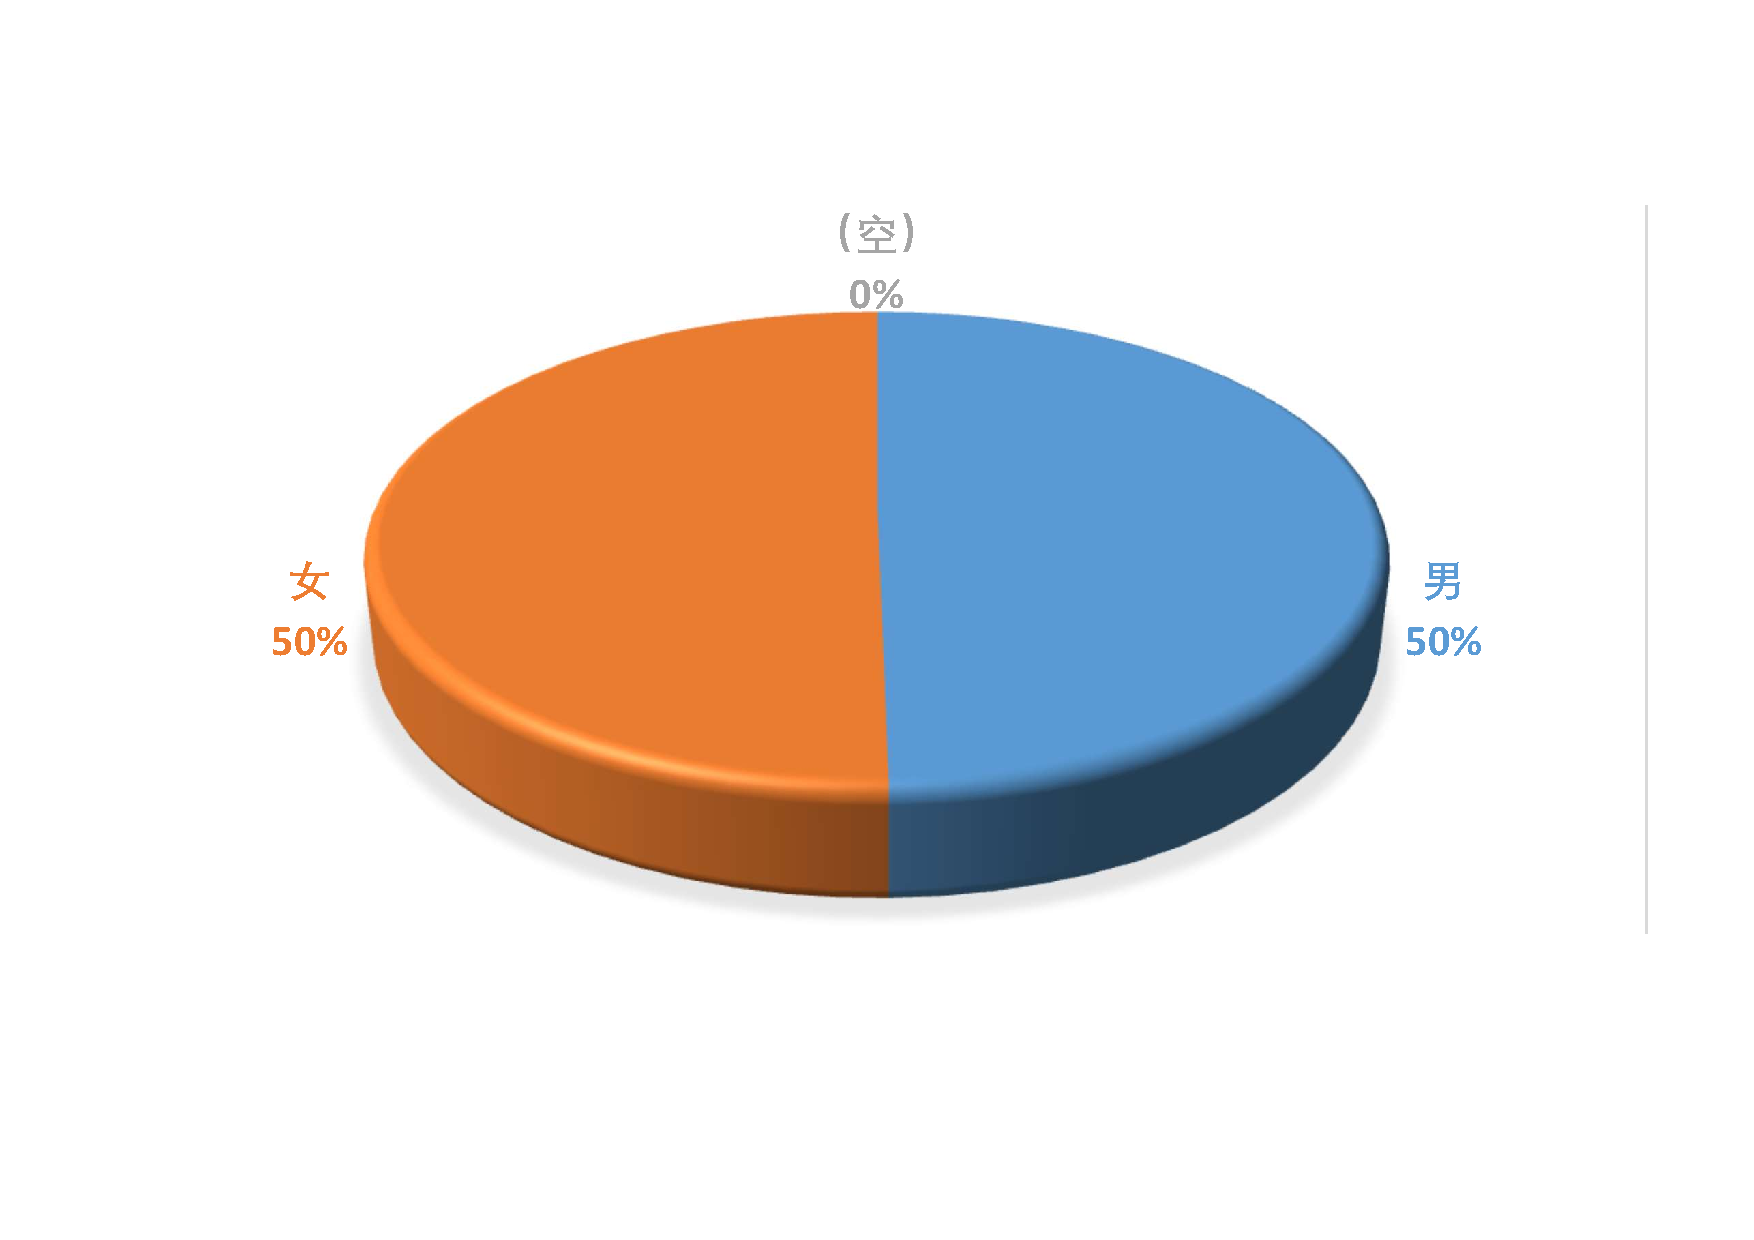
\includegraphics[width=0.35\textwidth]{figure/data/1.pdf}\
%\end{wrapfigure}
1.您的性别: \\
A.男\tabskips B.女
\par 该问卷的受访对象中,男女比例分别为49.70\%和50.30\%,比
较科学合理。其中,选项“(空)”表示受访者没有在该题作答,后面调查问题中出现的这个选项均表示这个含义。特此说明。后不赘述。
\par\noindent 2.您的年龄段:\\
A. 18岁以下\tabskips B. 18-25岁 \tabskips C. 26-35岁\tabskips D. 36-50岁\tabskips E. 50岁以上
\par 调查结果显示,在1491名受访者中,18岁以下
的受访者有74人,占总数的4.96\%:18—25岁的受访
者有661人,占总数的44.33\%;26-35岁的受访者有
435人,占总数的29.18\%:36—50岁的受访者有216人。
占总数的14.49\%;50岁以上的受访者有105人,占
总数的7.04\%。综上所述,18-25年龄段和26-35年
龄段的人数最多,两者总人数占受访者总数的比例高
达73.51\%。受访者年龄比例符合当前电影消费主体
趋于年轻化的趋势,有一定的代表性。

\begin{figure}[htbp]
  \centering
  \foreach \n in{1,...,5} {
  \begin{minipage}{0.49\textwidth}
    \includegraphics[width=\textwidth]{figure/data/\n.pdf}
  \end{minipage}
  }
\end{figure}

\par\noindent 3.您目前的职业:\\
A.学生 \tabskips B.农民 \tabskips C.机关和事业单位职工 \tabskips
D.工人 \tabskips E.自由职业者\tabskips F.其他
\par 调查结果显示,在1491名受访者中,学生、农民、
机关和事业单位职工、工人、自由职业者、其他的人
数分别为456、129、368、148、216、174,分别占
总数的30.58\%、8.65\%、24.68\%、9.93\%、14.49\%、 11.67\%。受访者中,所占比例由高到低排前三位的是
学生、机关和事业单位职工、自由职业者,三者所占
比例达69.75\%。
\par\noindent 4.请问您的文化程度:\\
A.初中或初中以下\tabskips  B.高中或中专 \tabskips C.大专\tabskips
D.本科 \tabskips  E.硕士 \tabskips F.博士
调查结果显示,在1491名受访者中,受访者的
文化程度所占比例由高到低排前三位的是本科、高中
或中专、大专,三者所占比例高达69.76\%。
\par\noindent 5.您目前的月收入:\\
A. 无收入  B.1000元以下
C.1000\textasciitilde 3000元 D.3000\textasciitilde5000元
E.5000\textasciitilde10000元  F.10000元以上
\par 调查结果显示,在1491名受访者中,受访者的
月收入主要集中在3000以下。其中,有37.83\%的受
访者表示月收入在1000\textasciitilde3000,有26.69\%的受访
者表示没有月收入,有14.49\%的受访者表示月收入
在1000以下。这一结果显然与受访者的职业构成相关。
\par {\heiti 小结:从各受访者的个人基本情况来看,此次问
卷调查受访对象的各方面结构是合理的,这也为问卷
调查的科学性奠定了基础。}

\subsection{电影消费的基本概况}
6. 您喜欢看电影吗? \\
A.喜欢 \tabskips B.一般 \tabskips C.不喜欢 \tabskips D.无所谓
\par
调查结果显示,有61.17\%的受访者表示喜欢看
电影,有31.45\%的受访者表示一般,而明确表示不
喜欢看电影的受访者只有3.76\%。这说明,电影作为
娱乐业的先锋还是很受大众青睐的。

\par\noindent 7. 您大约多长时间看一次电影:\\
A.一次/周  \tabskips B.一次/月 \tabskips C.一次/季度\tabskips
D.一次/年\tabskips E.一次/多年\tabskips F.没有看过\tabskips
G.每月多次\tabskips H.每周多次
\par 从调查表中可以看出,有33.20\%的受访者表示
每周看一次电影,有23.81\%的受访者表示每月看一
次电影,有11.07\%的受访者表示每季度看一次电影。
考虑到有9.99\%的受访者和5.57\%的受访者分别表
示每周多次和每月多次观影,则应当有一半左右的受
访者平均每周看一次电影。在消费娱乐方式的多样化
的今天,这一结果说明看电影仍然是一种主流的娱乐
方式。
\begin{figure}[htbp]
  \centering
  \foreach \n in{6,...,13} {
  \begin{minipage}{0.49\textwidth}
    \includegraphics[width=\textwidth]{figure/data/\n.pdf}
  \end{minipage}
  }
\end{figure}
\par\noindent 8. 您一般通过哪种方式看电影:\\
A.影院 \tabskips B.网络 \tabskips C.电视 \tabskips D.碟片\tabskips
E.手机\tabskips F.露天电影\tabskips G.其他途径

调查结果显示,受访者看电影的主要途径是网络、
电视和影院。其中,有高达51.44\%的受访者一般通
过网络看电影,有26.02\%的受访者一般通过电视看
电影,而只有9.79\%的受访者一般是通过影院看电影。
这说明网络和电视成为了最主要的观影途径,而传统
的影院地位则受到了很大的挑战。另外,除了有6.37\%
的受访者通过碟片看电影外,选择其它观影方式的人
数寥寥无几。这反映出受访者观影途径有集中化的趋
势,其它途径的观影方式有继续弱化的趋势。

\par\noindent 9.你通常是通过什么途径了解影片的信息(多选题)?\\
A.电视宣传\tabskips B.网络传播\tabskips C.朋友介绍\tabskips
D.海报宣传\tabskips E.报刊杂志\tabskips F.广播\tabskips G.其它
\par 调查结果显示,受访者主要是通过网络传播、电视
宣传和朋友介绍来了解影片信息的。选择这三种途
径的受访者分别占到了总数的53.86\%、47.42\%和
40.85\%。从调查结果中不难看出,由于网络的便利性,
网络传播的作用已经超过了传统的海报宣传和电视宣
传,成为第一大影片传播途径。但是,也应当看到,
传统的海报宣传和电视宣传还是具有很强的生命力。
这些宣传方式可以有效地弥补网络传播的不足。一个
值得关注的现象是朋友介绍在传播影片信息方面起到
了独特的作用。在现代信息社会中,多种信息传播途
径的建立使得人与人的沟通变得非常便利。这使得朋
友介绍成为传播影片信息的一个主要途径。
\par\noindent 10.如果你喜欢看一部电影,最主要是由于:\\
A.故事题材\tabskips B.演员阵容\tabskips C.导演\tabskips
D.制作规模\tabskips E.影评 \tabskips F.获奖情况

从调查结果来看,受访者喜欢看一部电影,主要
是由于故事题材和演员阵容。选择这两项的受访者分
别占到了总人数的46.61\%和31.66\%。而选择其它选
项的受访者比例明显偏低,没有一项的受访者比例超
过10\%。这反映出受访者对于故事题材吸引人、演员
阵容强大的影片有特殊的偏好,而对于像影评、导演、
制作规模和获奖情况等影片信息则关注很少。该调查
结果所反映出的信息对于影片的制作和宣传都有重要
参考价值。
\par\noindent 11.你喜欢看哪几种类型的电影(多选题)?\\
A.动作片\tabskips  B.爱情片\tabskips C.恐怖片\tabskips
D.喜剧片\tabskips E.伦理片\tabskips F.动画片\tabskips
G.文艺片\tabskips H.战争片\tabskips I.其他

\par 从上表可以看出,有一半左右的受访者表示喜欢
看喜剧片、爱情片和动作片,而其它类型影片的受欢
迎程度则很难与这三种类型的影片相比。这说明注重
感官刺激的娱乐性影片仍然是电影消费市场的主流影
片。这一结果与电影的娱乐化发展趋势相符合。从这
一调查结果不难看出,受访者普遍持有一种乐观的人
生态度。这与整个经济社会的蓬勃发展息息相关。在
其它类型影片中,受访者除了对伦理片和动画片的兴
趣相对较小外,对战争片、文艺片、恐怖片的兴趣则
相差不大。这说明电影在朝娱乐化发展的同时,也有
朝多样化发展的趋势。这符合社会的多元化发展潮流。

\par\noindent 12.你喜欢什么类型的影片结局?\\
A.完美大结局\tabskips B.悲剧结局 \tabskips
C.含蓄性结局\tabskips D.其他

\par 选择不同的结局可以反映一个人的性格特点。调
查结果显示有高达56.07\%的受访者选择了完美大结
局,这说明了大多数受访者持乐观的人生态度。该题
也印证了第11题的结论,即受访者普遍持有一种乐
观的人生态度。

\par\noindent 13.你喜欢看哪些国家或地区的电影:(多选题)\\
A.欧美\tabskips B.日韩 \tabskips C.大陆\tabskips
D.港台\tabskips E.泰国\tabskips F.其他
\par 调查结果显示,受访者主要喜欢看欧美和大陆
的电影。喜欢看欧美电影的受访者占总数的53.86\%,
而喜欢看大陆电影的受访者则占到了总数的52.05\%。
这说明,虽然欧美影片仍然受到市场的追捧,但是伴
随着国内电影消费市场的复苏,大陆影片一改往日的
颓势,其发展势头良好。
\par {\heiti 小结:从问卷调查结果来看,作为一种娱乐方式,
电影仍然受到消费者的广泛欢迎。当前,随着互联网
和电影制作技术的飞速发展,电影消费也呈现出一些
新特点。比如,互联网的发展促进了网络消费电影的
飞速发展,当前,有高达51.44\%的受访者表示是通
过网络来看电影的。此外,中国观众偏向于观看有完
美大结局的喜剧片、爱情片和动作片,关注影片的故
事题材和演员阵容,比较喜欢欧美片、大陆片和港
台片。}
\subsection{影院消费的基本概况}
\par\noindent 14. 您喜欢去电影院看电影吗?\\
A.喜欢\tabskips B.一般 \tabskips C.不喜欢\tabskips D.无所谓

\par 调查结果显示,明确表示喜欢去电影院看电影的
受访者比例最高,达到35.75\%,而明确表示不喜欢去
电影院看电影的受访者只占总数的11.94\%,但是表
示“一般”或。无所谓”的比重分别达到32.26\%和
18.31\%,这说明,随着娱乐形式和看电影方式的多样
化,人们对传统去电影院看电影的观念已经发生变化,
具体表现是有相当一部分受访者对去电影院看电影表
示“一般”或“无所谓”。

\par\noindent 15.您大约多长时间去电影院看一次电影?\\
A.一次/周\tabskips B.一次/月\tabskips C.一次/季度\tabskips
D.一次/年\tabskips E.一次/多年\tabskips F.没去过\tabskips
G.多次每月
\begin{figure}[htbp]
  \centering
  \foreach \n in{14,...,18} {
  \begin{minipage}{0.48\textwidth}
    \includegraphics[width=\textwidth]{figure/data/\n.pdf}
  \end{minipage}
  }
\end{figure}
\par 调查结果显示,当被问到大约多长时间去电影院
看一次电影时,受访者的意见比较不一致。表示没去
过电影院看电影的受访者人数最多,但其所占比例也
仅有19.92\%。跟第7题的调查结果相比,一个明显
的事实是受访者中的大多数人在大部分时候都不是在
电影院看电影的。
\par\noindent 16.您对影院基础设施和服务的满意程度:\\
A.非常满意\tabskips B.满意\tabskips C.一般\tabskips
D.不满意\tabskips E.太差,非常不满意

\par 调查结果显示,有高达49.33\%的受访者表示对
于影院基础设施和服务的满意程度感觉一般,而对于
影院基础设施和服务的满意程度感觉满意及非常满
意的受访者只占总数的28.7\%,另外选择不满意的受
访者比例只有4.85\%。这说明影院的基础设施和服务
都达到了一定水平,要想再进一步提高确实有一定
的困难。

\par\noindent 17.若您不愿意去电影院看电影,理由可能是(多
选题):\\
A.时间问题\tabskips B.交通不便\tabskips C.票价过高\tabskips
D.电影院硬件设施差\tabskips E.所在地没有影院\tabskips
F.其他


\par 调查结果显示,受访者不愿意去电影院观看电影
的理由主要是时间问题、票价过高和交通不便,选择
这三项的受访者分别占到了总数的47.08\%、43.33\%
和18.65\%。这说明,一方面相对于过高的票价,受
访者更加关注时间问题:另一方面交通不便及所在地
没有影院也影响了受访者去影院消费。

\par\noindent 18.促使您去电影院看电影的原因是(多选题):\\
A.能看到最新上映的电影\tabskips B.影院气氛好\tabskips
C.交友交际\tabskips  D.影院视听效果好\tabskips
E.广告宣传\tabskips  F.其他

\par 调查结果显示,受访者去电影院看电影的主要
原因是影院气氛好、影院视听效果好及能看到最新上
映的电影,选择这三项的受访者分别占到了总数的
40.44\%、38.43\%和38.03\%。这说明受访者去影院观
看电影主要追求观影的气氛、视听享受以及观看最新
影片的新鲜感。
\par {\heiti
小结:从问卷调查结果来看,随着娱乐形式和看
电影方式的多样化,人们对传统去电影院看电影的观
念已经发生变化,具体表现是有相当一部分受访者对
去电影院看电影表示“一般”或“无所谓”。影响观众
走进电影院看电影的主要原因是时间问题、票价过高
和交通不便。受访者去电影院看电影的主要原因是影
院气氛好、影院视听效果好及能看到最新上映的电影。
}
\subsection{受访者对票价和促销的一般态度}
\par\noindent 19.您平均每月用在文化娱乐方面的支出为:\\
A.100元以下\tabskips B.100\textasciitilde200元\tabskips
C.200\textasciitilde 300元\tabskips D.300\textasciitilde400元\tabskips
E.400元以上
\par 该题目的目的是调查出受访者每月用于文化娱乐
方面的总支出。有高达84.24\%的受访者每月用在文
化娱乐方面的支出为300元以下,其中,45.21\%的
受访者的支出在100元以下。这说明绝大多数受访者
每月用在文化娱乐方面的总支出不高。其可能的原因
有:一是受访者总收入不高;二是电视和网络提供了大
量的娱乐节目,这种近乎免费的娱乐方式对于部分高
价的娱乐消费形成了替代作用。

\par\noindent20.请问您每月用于看电影上的支出为:\\
A.30元以下\tabskips B、30\textasciitilde60元\tabskips
C.60\textasciitilde100元 \tabskips D、100\textasciitilde150元\tabskips
E.150元以上
\par 本题承接上题而设置,目的是调查出受访者在每
月用于文化娱乐方面的支出中有多少是电影支出。调
查显示,有82.82\%的受访者每月用于看电影的支出
在60元以下,且有59.30\%的受访者每月用于看电影
的支出在30元以下。
\begin{figure}[htbp]
  \centering
  \foreach \n in{19,...,22} {
  \begin{minipage}{0.48\textwidth}
    \includegraphics[width=\textwidth]{figure/data/\n.pdf}
  \end{minipage}
  }
\end{figure}
\par\noindent21.您认为当前我国影院电影票价:\\
A.太高\tabskips B.较高\tabskips C.适中\tabskips D.较低
\par 从调查结果不难看出,有接近一半的受访者表
示票价较高,而认为票价较低的受访者只占总人数的
1.34\%。这说明受访者普遍认为票价偏高。当然,也
应当看到有29.18\%的受访者认为当前票价适中。这
说明消费市场已经呈现出分化的趋势,即不同层次的
观众对价格的敏感程度是不同的。如何满足不同层次
观众的观影需求是扩大电影消费的关键。
\par\noindent22.请问您认为一部电影的合理定价应该在:\\
A.10元以下\tabskips
B.10\textasciitilde 20元\tabskips
C.20\textasciitilde30元\tabskips  D.30\textasciitilde 40元\tabskips
E.40\textasciitilde50元\tabskips
F.50元以上
\par 调查结果显示,在1491名受访者中,有86.19\%
的受访者认为合理的电影票价在40元以下。这说明
大多数受访者可以接受40元以下的票价。2016年全
国的电影平均票价是33.2元,正处于这一合理价
格区间。可以说,我国电影消费近年来的繁荣是与合
理的票价不无相关的。但是,从调查结果中也应当看
到,有多达41.52\%的受访者认为合理的电影票价在
20\textasciitilde30元之间。这说明适当地降低票价将有助于吸
引这部分观众走进影院。

\par\noindent23.请问一部您喜欢的电影,您最多愿意支付多
少钱来购买电影票?
A.20元以下\tabskips
C.30\textasciitilde50元\tabskips
B.20\textasciitilde30元\tabskips
D.50元以上

\par 本题承接上题而进行设置,目的是在调查出合
理票价的同时,调查一下受访者对自己喜欢的影片究
竟愿意支付多少钱来购买电影票。调查结果显示,在
1491名受访者中,选择20\textasciitilde30元选项的受访者人
数最多,占总人数的38.56\%;选择20元以下选项的
人数次之,占总人数的32.26\%:选择30\textasciitilde50元选项
的人数又次之,占总人数的19.79\%。由此可以看出,
观众普遍认为为自己喜欢的电影多支付一定数额的钱
来购票是值得的。这也说明了影片质量对于电影消费
的巨大影响。如果影片质量过硬且符合观众的口味,
现行票价就不会是制约电影消费的主要问题。每到大
片放映时一票难求的火爆场面就是对此最好的证明。
因此,提高影片质量是促进电影消费的永恒话题。
\begin{figure}[htbp]
  \centering
  \foreach \n in{23,...,26} {
  \begin{minipage}{0.48\textwidth}
    \includegraphics[width=\textwidth]{figure/data/\n.pdf}
  \end{minipage}
  }
\end{figure}
\par\noindent24.如果电影价格再提高一倍,您会放弃看电影
而选择其它娱乐方式吗?\\
A.不会\tabskips B.会\tabskips C.不知道

\par 可以看出,在1491名受访者中,当被问
到如果电影价格再提高一倍、是否会放弃看电影而选
择其它娱乐方式时,有53.72\%的受访者表示会放弃
看电影而选择其它娱乐方式,有30.52\%的受访者表
示不知道,而只有11.86\%的受访者表示不会放弃看
电影。这再次说明观众呈现出分化的趋势。由于个人
偏好和个人收入的不同,相同的票价对于不同观众的
意义是不同的。对于偏爱电影消费和个人收入较高的
观众而言,较高的票价是可以接受的:但对于个人收入
不高的观众而言,过高的票价就成为了阻碍电影消费
的壁垒。放弃看电影而选择其它娱乐方式就是这部分
观众的最佳选择。

\par\noindent25.您会选择在优惠活动日去看电影吗?\\
A.会\tabskips B.不会\tabskips C.无所谓\tabskips D.不知道

\par 从调查结果中可以看出,虽然有43.73\%的受
访者表示会在优惠活动日去看电影,但是也有高达
31.59\%的受访者表示无所谓。这表明虽然优惠活动
日对刺激电影消费有一定的作用,但是作用没有想像
中那么大。观众走进影院观看电影主要考虑的还是一
个综合因素。
\par\noindent26.请问哪种电影营销方式最能吸引您:
A.票价折扣\tabskips
B.派发精美纪念品\tabskips
C.购物赠票\tabskips D.买一送一

\par 调查结果显示,在1491名受访者中,有38.10\%
的受访者表示票价折扣最有吸引力,有27.70\%的
受访者表示购物赠票最有吸引力。而有18.44\%和
12.41\%的受访者分别表示派发精美纪念品和买一送一
最有吸引力。如果把买一送一也看作是一种类型的票
价折扣,则倾向于票价折扣的受访者占到了总人数的
50.51\%。这说明对一半左右的受访者而言,票价折扣
是最实惠的,也是最有吸引力的。但是,也应当看到,
有相当一部分受访者选择了购物赠票和派发精美纪念
品。这表明不同观众对于不同的电影营销方式有不同
的偏好。因此,为了取得最优的营销效果,应当在立
足票价折扣的基础上,大力开发各种电影营销方式,
以期刺激各种类型观众的消费需求。
\par {\heiti
小结:从问卷调查结果来看,受访者在文化娱乐
方面的总支出并不高,有高达84.24\%的受访者每月
用在文化娱乐方面的支出为300元以下。同样地,受
访者在电影消费方面的支出也不高,有82.82\%的受
访者每月用于看电影的支出在60元以下,这主要与
受访者的收入和消费习惯有关。与受访者在电影消费
方面的低支出相对应的是受访者普遍认为票价偏高。
从受访者对营销方式的偏好上可以看出,受访者更倾
向于票价折扣这类比较实惠的电影促销方式。
}
\begin{figure}[htbp]
  \centering
  \foreach \n in{27,...,29} {
  \begin{minipage}{0.48\textwidth}
    \includegraphics[width=\textwidth]{figure/data/\n.pdf}
  \end{minipage}
  }
\end{figure}
\subsection{受访者对国产影片的态度}
\par\noindent 27.国产影片与国外影片的质量相比,您认为\\
A.国产影片的质量更好\tabskips
B.国外影片的质量更好\tabskips
C.两者质量差不多 \tabskips D.没感觉
\par 调查结果显示,在1491名受访者中,被受访者
关注的前三个选项分别是“国外影片的质量更好”、“没
感觉”和。两者质量差不多”,选择这三项的受访者分
别占到了总数的49.23\%、19.18\%和18.24\%。这表
明受访者还是更加认可国外影片的质量。
\par\noindent 28.你认为中国影片的质量是:\\
A.越来越好\tabskips
B.逐渐衰退\tabskips
C.有的好有的糟糕\tabskips D.难以评价

\par 可以看出,有40.11\%的受访者认为国产
影片的质量会越来越好,有37.76\%的受访者则认为
国产影片有的好有的糟糕。这表明一方面观众对于国
产影片近年的快速发展给予了肯定,并且对国产影片
质量的提高有较强的期待,另一方面观众对于国产影
片质量良莠不齐的现象有较深刻的认识。

\par\noindent 29.你认为国产影片和国外影片的差别在于:(多
选题)\\
A.故事情节\tabskips  B.演员演技\tabskips C.演员阵容\tabskips
D.电影拍摄技术\tabskips E.营销手段 \tabskips F.导演\tabskips
G.其他

\par 调查结果显示,在1491名受访者中,被受访者
关注的前三个选项分别是。故事情节”、“电影拍摄技
术”和“演员演技”,选择这三项的受访者分别占到了
总数的54.12\%、52.05\%和34.94\%。从这样的结果中,
一方面可以看出观众是从哪几个方面来界定一部高质
量影片的,这有助于制片方有针对性地改菩国产影片
质量;而另一方面则可以看出观众对于故事情节和电
影画面质量有较高的要求。这说明观众倾向于观看追
求感官享受的娱乐性影片。
\par {\heiti
小结:从问卷调查结果来看,受访者对国产影片
的质量有较高的期待,并且认为国产影片和国外影片
的差别主要在故事情节、电影拍摄技术和演员演技方
面。这对把握国产影片今后的发展方向有重要价值。
}

\subsection{其它方面}
\par\noindent 30.如果送您两张电影票,请问您最愿意邀请谁同去:\\
A.恋人\tabskips B.家人\tabskips C.朋友\tabskips D.其他人
\par 该题是一个关于电影促销的问题,目的是调查出
受访者更倾向于同谁一起观看电影。调查结果显示,
当被问到如果获赠两张电影票、最愿意邀请谁共同观
影时,有38.43\%的受访者表示最愿意邀请恋人共同
观影,有30.52\%的受访者表示最愿意邀请家人共同
观影,而表示最愿意邀请朋友共同观影的受访者也占
到了26.02\%。这说明观众倾向于与身边的恋人、家
人和朋友结伴共同观影。调查结果将有助于院线公司
根据不同影片而采取不同的促销策略。
\par\noindent 31.您购买的影碟中盗版影碟所占的比例为:\\
A.10\%以下\tabskips
B.10\%\textasciitilde30\%\tabskips
C.30\%\textasciitilde50\%\tabskips  D.50\%\textasciitilde80\%\tabskips
E.80\%\textasciitilde100\%

\par 调查结果显示,选择80\%\textasciitilde100\%和30\%\textasciitilde50\%等
选项的人数最多,其比例分别为26.76\%和19.85\%。
虽然有26.76\%的受访者表示他们所购买的影碟中盗
版影碟所占的比例为80\%\textasciitilde100\%,但是选择其它选项
的受访者也不在少数。这说明,与前些年相比,近年
来在政府的大力整顿下,影碟盗版现象得到了有效遏
制,电影消费环境有了明显改善。

\par\noindent 32.您会购买与电影相关的各种产品吗:\\
A.会\tabskips B.可能会\tabskips C.不确定\tabskips D.不会
调查结果显示,明确表示不会购买电影相关产品
的受访者只占总数的24.61\%。虽然明确表示会购买
电影相关产品的受访者只占总数的10.26\%,但是有
相当一部分受访者对此持观望态度。这说明只要电影
相关产品能够最大限度满足顾客的需要,其市场前景
就一定很广阔。

\par\noindent 33.您会购买与电影相关的下列哪些产品:(多选题)\\
A.DVD或者VCD碟片\tabskips B.相关书籍\tabskips
C.游戏\tabskips D.玩具\tabskips E.服装\tabskips F.海报\tabskips
G.文具\tabskips H.装饰物\tabskips I.其他

\par 该题是一道多项选择题,目的是调查出受访者
对电影相关产品的消费偏好。调查结果显示,有高
达48.36\%的受访者表示会购买DVD或者VCD:有
24.75\%的受访者和23.41\%的受访者分别表示会购买
装饰物和相关书籍。对于其它电影相关产品,有意向
购买的受访者比例则差不多。这反映出,一方面传统
的影碟仍然是人们消费电影产品的主要产品,另一方
面其它电影相关产品的受欢迎程度则差不多。这说明,
与西方国家高度发达的电影产品消费市场相比,我国
电影产品消费市场还很弱小,还需要进一步的培育和
发展。
\par {\heiti
小结:考虑到电影的相关产品市场有待进一步开发,
并且有相当一部分盗版电影挤占了正版影片的市场,
我国的电影消费市场的开发仍然任重而道远。
}
\begin{figure}[htbp]
  \centering
  \foreach \n in{30,...,33} {
  \begin{minipage}{0.48\textwidth}
    \includegraphics[width=\textwidth]{figure/data/\n.pdf}
  \end{minipage}
  }
\end{figure}
\section{总结与启示}
综合分析此次问卷调查数据结果显示。在近年来
居民可支配收入较快增长的情况下,随着居民消费结
构升级方兴未艾,青年观众正逐渐将电影消费发展为
一种习惯性的娱乐方式,国内电影消费的空间正在逐
步扩大,但是与西方国家高度发达的电影产品消费市
场相比,我国电影产品消费市场还很弱小,还需要进
一步的培育和发展,我国电影消费市场正进入一个新
的发展阶段。
\par 从电影消费的群体特征来看,目前,我国电影消
费群体呈现年轻化态势,具有大中专以上学历的年轻
观众成为电影消费的固定群落,且这部分群体以学生、
机关或事业单位职工、自由职业者的身份为主,拥有
相对较低的收入水平,希望与恋人、家人或朋友一起
观影,表明了居民消费结构升级过程中,消费理念的
转变和超前在对电影消费群体的重要影响。
\par 从电影消费的群体需求来看,尽管消费娱乐方式
正日趋多样化,但是电影消费娱乐仍然大受青睐,仍是
主流的娱乐方式、娱乐业的先锋。注重感官刺激的娱乐
性影片是电影消费市场的主流影片,如喜剧片、爱情片、
动作片以及影片的故事题材、演员阵容成为电影消费
的重要看点,表明了我国电影消费中呈现出的娱乐化
趋势。同时,虽然欧美影片仍受市场追捧,但是在国
内电影消费市场扩张的情况下,高质量的国产影片正
一改往日的颓势,得到国内观众的肯定,表明了能否
满足观众娱乐性需求成为电影消费需求的重点。
\par 从电影消费的具体途径来看,我国电影消费方式
呈现集中化的趋势,网络、电视、影院成为电影消费
的主要方式,而其他观影方式继续弱化。其中,追求
观影的气氛、视听的享受、最新影片的新鲜感等因素,
是促使观众去电影院看电影的主要动力。
\par 从电影消费的影响因素来看,影响居民电影消费
的重要因素呈现分化趋势,总体来说,娱乐时间、电
影票价、交通状况成为影响电影消费的重要因素。由
于个人偏好、收入水平等方面的差异,不同的观众对
电影消费表现出不同的要求。在当前文化娱乐消费支
出整体不高的情况下,以及其他娱乐消费方式的发展,
大部分观众难以接受高票价,票价成为阻碍电影消费
的核心壁垒。但是,影片质量过硬且符合观众的口味,
往往促使观众忽视高票价的影响。
\par 由此可以得到如下启示:
\par\noindent {\fangsong 1. 注重电影的网络宣传,形成良好的口碑传播}
\par 数据显示,新生代了解电影资讯的主要途径来源
于网络。因此,电影营销应更加注重网络宣传,在新生代消费者中形成良好的口碑。
网络传播与口碑相传是针对新生代最为精准有效的营销方式。
\par\noindent {\fangsong 2.降低电影票价,创新促销方式}
\par 调查显示,目前电影的票价超过了新生代消费者的承受能力,阻碍了更多新生代消费者进入电影院, 降低了他们去电影院观看电影大片的频率。因此,可 以通过多元化的促销方式来降低电影票价。首先,多数新生代都不是单独去电影院的,他们通常会约上男(女)朋友、同学亲友,因此,影院可以适当为他们 提供优惠套累;其次,年轻人时下流行网络团购,电 影院可以用优惠的价格将多部电影捆绑销售;再次, 电影院还可以与多家商户合作开展联合促销,联合发行优惠卡,对各商户的会员实行优惠(如:银行信用卡、南航明珠卡、各商场会员卡等);最后,电影院还可以适当延长优惠时段,提高优惠时段的折扣比例。这些小小的优惠举惰,无疑都将对价格敏感的新 生代消费者产生巨大的吸引力。
\par\noindent {\fangsong 3.采取多元化的电影售票方式}
\par 当前,许多人购买电影票仍然是在电
影院现场购票。一方面,这可能需要提前到场排队购买,造成不必要的时间浪费;另一方面,可能因为当 日热门电影场次不足,导致错失喜爱的影片。因此,
电影院的售票方式也应当针对新生代消费者的德求更为灵活多样。例如,可以通过网络售票、电话售琪、 电子票、手机支付等多种售票方式方便购买,以赢得 更多的消费者。
\end{document}
